\documentclass[UTF8,a4paper,11pt,fontset=fandol]{ctexart}
\usepackage[margin=23mm]{geometry}
\usepackage{amsmath,amssymb,booktabs,longtable,graphicx,float,fancyhdr,xcolor,needspace}
\usepackage{xurl}
\usepackage[unicode,colorlinks=true,linkcolor=black,urlcolor=blue]{hyperref}
\definecolor{accent}{HTML}{155574}
\pagestyle{fancy}
\fancyhf{}
\fancyhead[L]{\small 数学建模训练论文}
\fancyhead[R]{\small 待人工审阅}
\fancyfoot[C]{\thepage}
\setlength{\headheight}{15pt}
\setlength{\parskip}{0.35em}
\setlength{\emergencystretch}{3em}
\title{\bfseries 有限资源下的整数生产配置与容量情景分析}
\author{}
\date{}
\begin{document}
\maketitle
\vspace{-2.4em}
\begin{center}\small\color{accent}训练草稿：计算已核验，建模解释、引用及赛事格式仍需队员审阅\end{center}
\begin{abstract}
针对有限工时与材料下的生产配置问题，建立带产量上下界的整数线性规划模型，并设置可行贪心方案作为比较基线。本次求解得到总利润 605.00，基线总利润为 515.00，相对变化为 17.48\%。通过逐项约束复算、线性松弛上界和小规模枚举交叉检验验证主方案，并比较资源同步变化的情景。结论限于已声明的教学数据与线性假设。
\end{abstract}
\noindent\textbf{关键词：}整数规划；资源配置；敏感性分析；可复现计算

\section{问题分析与数据来源}
本案例使用人工构造的教学数据，用于验证建模、代码与论文的一体化流程；不是企业实测数据，也不是历年赛题附件。
\begin{description}

\item[Q1] 在资源和产量上限约束下，确定使总利润最大的整数生产方案。

\item[Q2] 分析资源容量同步下降和上升时的方案目标值，并讨论适用边界。

\end{description}

\section{模型假设与符号}
\begin{enumerate}

\item 每种产品的单位利润、工时和材料消耗在本次决策期内保持不变。

\item 产品数量为非负整数，产量上限由附件给定，未销售风险未计入。

\item 情景分析中全部资源容量按同一比例变化，其余参数保持不变。

\end{enumerate}
\begin{longtable}{p{.16\textwidth}p{.46\textwidth}p{.20\textwidth}}
\toprule 符号 & 含义 & 单位 \\ \midrule

x\_1 & 产品甲 & 件 \\

x\_2 & 产品乙 & 件 \\

x\_3 & 产品丙 & 件 \\

\bottomrule
\end{longtable}

\section{模型建立与求解方法}
决策变量是整数，目标和资源约束均线性；使用 MILP 并与线性松弛上界比较。

\begin{equation}
\max\; z=\sum_{j=1}^{n}p_jx_j
\end{equation}

\begin{equation}
\sum_{j=1}^{n}a_{ij}x_j\leq b_i\quad(i=1,\ldots,m)
\end{equation}

\begin{equation}
l_j\leq x_j\leq u_j,\quad x_j\in\mathbb{Z}_{\geq0}
\end{equation}

\noindent\textbf{基线方案：}从最低产量出发，按单位归一化资源利润贪心增量配置；若最低产量不可行则报告不可行。


\section{主方案与基线比较}
以产品数量为决策变量，使用混合整数线性规划求解器完成优化[scipy\_milp]。主方案总利润为 605.00，贪心基线为 515.00，相对变化为 17.48\%。线性松弛上界为 605.00。具体产品数量列于配置表；最优性表述以求解状态和交叉核验记录为依据。

\section{容量情景与决策解释}
分别对资源容量实施同步收缩与扩张并重新求解，具体目标值和状态列于情景表。该实验反映给定方向上的局部响应，整数生产数量可能导致目标值随容量呈现阶梯变化。资源类别的边际价值需要分别扰动后进一步分析。


\section{计算结果与图表}
所有数值均读取同一次实验记录；表中的不可用项保留其原始状态。

\Needspace{7\baselineskip}
\subsection*{生产配置方案}
{\small
\begin{longtable}{lll}
\toprule
产品 & 数量 & 利润 \\ 
\midrule\endhead

产品甲 & 9 & 360 \\ 

产品乙 & 7 & 245 \\ 

产品丙 & 0 & 0 \\ 

\bottomrule
\end{longtable}}

\Needspace{7\baselineskip}
\subsection*{资源容量情景}
{\small
\begin{longtable}{lll}
\toprule
容量倍率 & 求解状态 & 目标值 \\ 
\midrule\endhead

0.9 & 最优 & 530 \\ 

1 & 最优 & 605 \\ 

1.1 & 最优 & 645 \\ 

\bottomrule
\end{longtable}}


\begin{figure}[H]
\centering
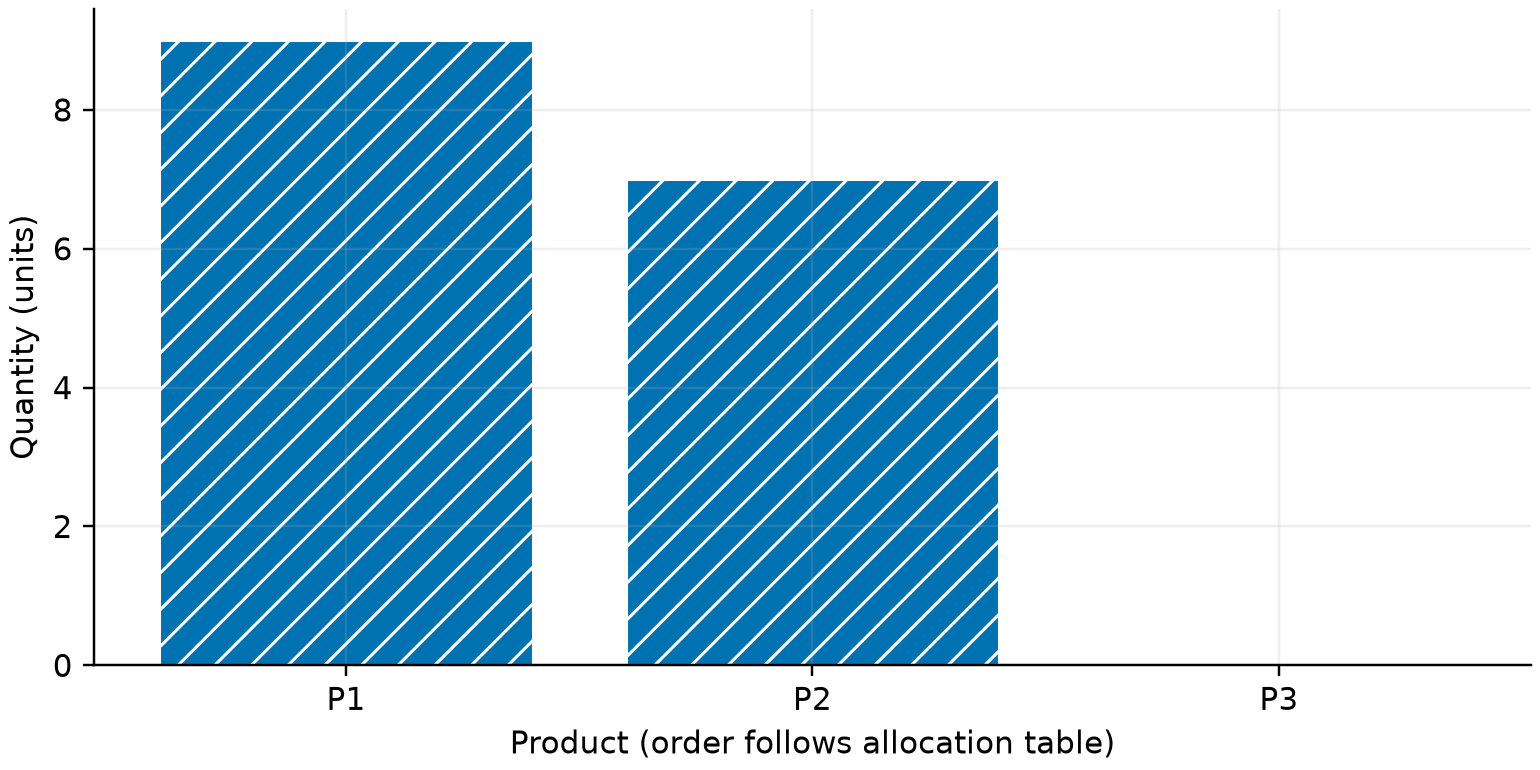
\includegraphics[width=.91\textwidth]{../figures/allocation.png}
\caption{各产品的整数配置数量；产品顺序与配置表一致。}
\end{figure}

\begin{figure}[H]
\centering
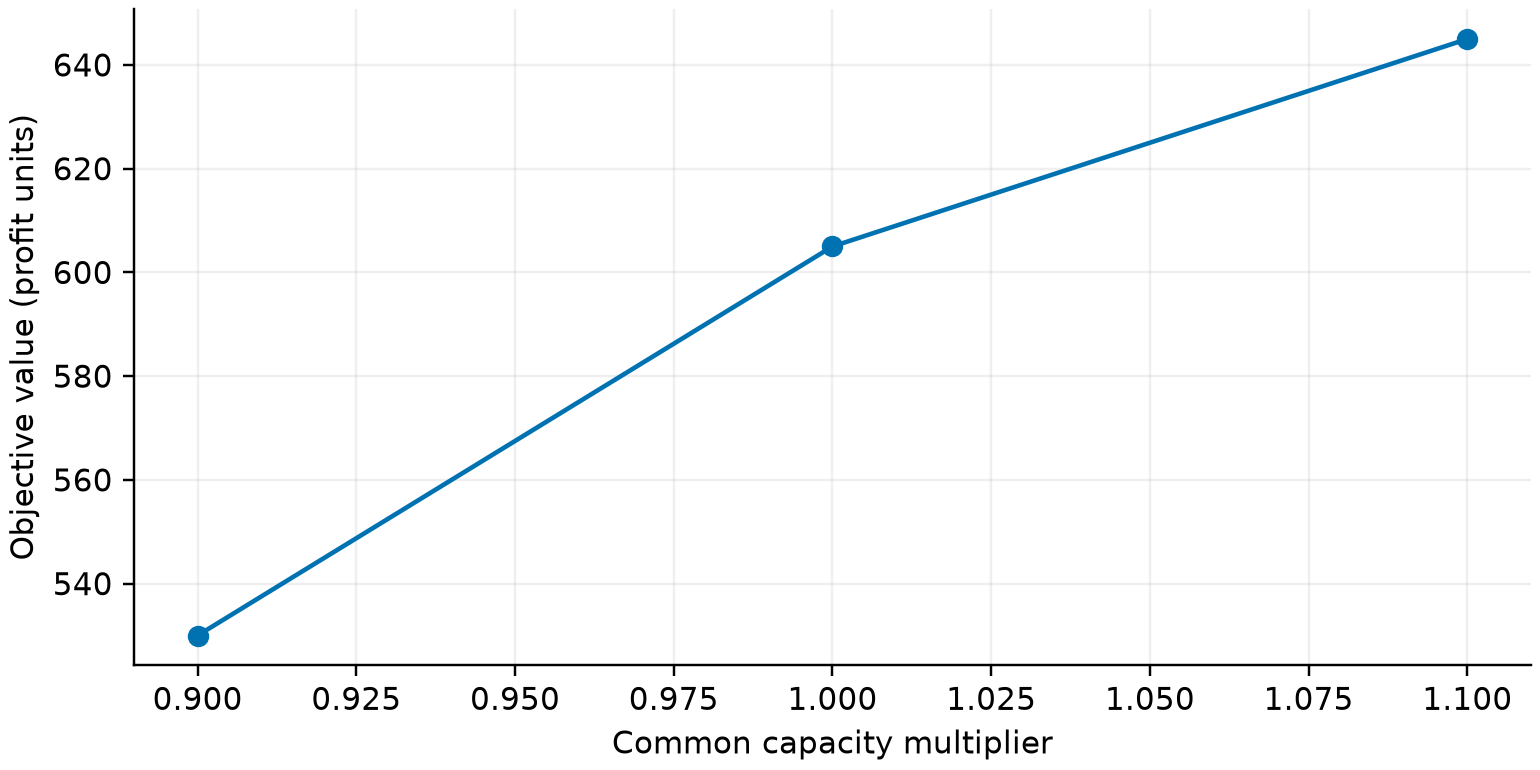
\includegraphics[width=.91\textwidth]{../figures/sensitivity.png}
\caption{全部资源容量同步变化时的目标值；不可行情景不绘制数值。}
\end{figure}


\section{检验、局限与改进方向}
本次自动核验覆盖了已编码的数值条件。自动核验通过不等价于题意解释已经充分，队员仍需对照原题审阅假设与结论。
\begin{itemize}

\item 利润与资源消耗视为常数，未包含价格反馈。

\item 情景扰动属于局部分析，不代表随机鲁棒最优。

\end{itemize}

\section*{参考来源}

\begin{description}

\item[scipy\_milp] SciPy 官方文档：混合整数线性规划 milp. \url{https://docs.scipy.org/doc/scipy/reference/generated/scipy.optimize.milp.html}. 核验状态：opened\_by\_agent.

\end{description}

\section*{复现与 AI 使用说明}
数据来源、程序版本和输入摘要见工作区中的 provenance.json；运行命令见复现说明。
本案例使用已声明的训练数据，结论仅用于演示建模过程。
实际 AI 工具使用、人工修改及核验记录保存在 ai\_usage.jsonl 中，由队员据实补充后按赛事要求整理。
\end{document}